%%%%%%%%%%%%%%%%%%%% author.tex %%%%%%%%%%%%%%%%%%%%%%%%%%%%%%%%%%%
%
% sample root file for your "contribution" to a contributed volume
%
% Use this file as a template for your own input.
%
%%%%%%%%%%%%%%%% Springer %%%%%%%%%%%%%%%%%%%%%%%%%%%%%%%%%%


% RECOMMENDED %%%%%%%%%%%%%%%%%%%%%%%%%%%%%%%%%%%%%%%%%%%%%%%%%%%
\documentclass[graybox]{svmult}

% choose options for [] as required from the list
% in the Reference Guide

\usepackage{type1cm}        % activate if the above 3 fonts are
                            % not available on your system
%
\usepackage{makeidx}         % allows index generation
\usepackage{graphicx}        % standard LaTeX graphics tool
                             % when including figure files
\usepackage{multicol}        % used for the two-column index
\usepackage[bottom]{footmisc}% places footnotes at page bottom


\usepackage{newtxtext}       % 
\usepackage{newtxmath}       % selects Times Roman as basic font

\usepackage{url} % Use the package "url.sty" to avoid problems with special characters used in your e-mail or web address

% MY ADDENDA
\usepackage{enumitem} %roman numbers
\usepackage[super]{nth} % for dates
\usepackage{verbatim}   % \begin and \end {comment}
\usepackage{hyperref}   % to use \href


% see the list of further useful packages
% in the Reference Guide

\makeindex             % used for the subject index
                       % please use the style svind.ist with
                       % your makeindex program

%%%%%%%%%%%%%%%%%%%%%%%%%%%%%%%%%%%%%%%%%%%%%%%%%%%%%%%%%%%%%%%%%%%%%%%%%%%%%%%%%%%%%%%%%
\begin{document}

\title*{An Agent-Based Model of COVID-19 Diffusion to Plan and Evaluate Intervention Policies}
\titlerunning{An Agent-Based Model of COVID-19 Diffusion}
% Use \titlerunning{Short Title} for an abbreviated version of
% your contribution title if the original one is too long
\author{Gianpiero Pescarmona, Pietro Terna, Alberto Acquadro, Paolo Pescarmona, Giuseppe Russo, Emilio Sulis, and Stefano Terna}
\authorrunning{G. Pescarmona, P. Terna\textit{et al.}}
% Use \authorrunning{Short Title} for an abbreviated version of
% your contribution title if the original one is too long
\institute{G. Pescarmona \at University of Torino, Italy, \email{gianpiero.pescarmona@unito.it}
\and P. Terna \at University of Torino, Italy; Fondazione Collegio Carlo Alberto, Italy \email{pietro.terna@unito.it}
\and A. Acquadro \at University of Torino, Italy \email{alberto.acquadro@unito.it}
\and P. Pescarmona \at University of Groningen, The Netherlands \email{p.p.pescarmona@rug.nl}
\and G. Russo \at Centro Einaudi, Torino, Italy \email{russo@centroeinaudi.it}
\and E. Sulis \at University of Torino, Italy; \email{emilio.sulis@unito.it}
\and S. Terna \at \url{tomorrowdata.io} \email{stefano.terna@tomorrowdata.io}
}
%
% Use the package "url.sty" to avoid
% problems with special characters
% used in your e-mail or web address
%
\maketitle

\abstract*{A model of interacting agents, following plausible behavioral rules into a world where the Covid-19 epidemic is affecting the actions of everyone. The model works with (i) infected agents categorized as symptomatic or asymptomatic and (ii) the places of contagion specified in a detailed way. The infection transmission is related to three factors: the characteristics of both the infected person and the susceptible one, plus those of the space in which contact occurs. The model includes the structural data of Piedmont, an Italian region, but we can easily calibrate it for other areas. The micro-based structure of the model allows factual, counterfactual, and conditional simulations to investigate both the spontaneous or controlled development of the epidemic.\newline\indent
The model is generative of complex epidemic dynamics emerging from the consequences of agents' actions and interactions, with high variability in outcomes, but frequently with a stunning realistic reproduction of the successive contagion waves in the reference region. 
There is also an inverse generative side of the model, coming from constructing a meta-agent optimizing the vaccine distribution among people groups---characterized by age, fragility, work conditions---to minimize the number of symptomatic people, using genetic algorithms.}

\abstract{A model of interacting agents, following plausible behavioral rules into a world where the Covid-19 epidemic is affecting the actions of everyone. The model works with (i) infected agents categorized as symptomatic or asymptomatic and (ii) the places of contagion specified in a detailed way. The infection transmission is related to three factors: the characteristics of both the infected person and the susceptible one, plus those of the space in which contact occurs. The model includes the structural data of Piedmont, an Italian region, but we can easily calibrate it for other areas. The micro-based structure of the model allows factual, counterfactual, and conditional simulations to investigate both the spontaneous or controlled development of the epidemic.\newline\indent
The model is generative of complex epidemic dynamics emerging from the consequences of agents' actions and interactions, with high variability in outcomes, but frequently with a stunning realistic reproduction of the successive contagion waves in the reference region. 
There is also an inverse generative side of the model, coming from constructing a meta-agent optimizing the vaccine distribution among people groups---characterized by age, fragility, work conditions---to minimize the number of symptomatic people, using genetic algorithms.}

%%%%%%%%%%%%%%%%%%%%%%%%%%%%%%%%%%%%%%%%%%%%%%%
%%%%%%%%%%%%%%%%%%%%%%%%%%%%%%%%%%%%%%%%%%%%%%%
\section{A quick introduction to epidemic modeling}
\label{intro}

The starting point is a compartmental model with Susceptible, Infected, and Recovered people (S.I.R.), but adding both a more detailed breakdown of the subjects involved in the contagion process \cite{Scala:2020aa} and a multi-scale framework to account for the interaction at different dimensional, and spatial levels \cite{doi:10.1142/S0218202520500323}. From the virus micro-level, we move to individuals and up to the collective behavior of the population.

Following \cite{rahmandad2008heterogeneity}, we know that the analysis based on the assumption of heterogeneity strongly differs from S.I.R. compartmental structures modeled by differential equations. Their work ponders when it is better to use agent-based models and when it would be better to use differential equation models. Differential equation models assume homogeneity and perfect mixing of characteristics within compartments, while agent-based models can capture heterogeneity in agent attributes and the structure of their interactions. We follow the second approach.

\begin{itemize}

\item

The model works with: 

\begin{enumerate}[label=\roman*]
\item infected agents categorized as symptomatic or asymptomatic and 
\item the places of contagion specified in a detailed way, thanks to agent-based modeling capabilities. 
\end{enumerate}

 \item
The infection transmission is related to three factors: the infected person's characteristics and those of the susceptible one, plus those of the space in which a contact occurs.

\end{itemize}


Finally, we subscribe the call of \cite{squazzoni2020} to <<cover the full behavioural and social complexity of societies under pandemic crisis>> and we work arguing that <<the study of collective behavior must rise to a ``crisis disciplin'' just as medicine, conservation, and climate science have, with a focus on providing actionable insight to policymakers and regulators for the stewardship of social systems>>, as in \cite{Bak-Colemane2025764118}. 

%%%%%%%%%%%%%%%%%%%%%%%%%%%%%%%%%%%%%%%%%%%%%%%
\subsection{Why model? Why agents? Why another model?}
\label{why}

Why another model, and most of all, why model? With \cite{epstein2008model}:
\begin{quote}
The choice (\ldots) is not whether to build models; it's whether to build explicit ones. In explicit models, assumptions are laid out in detail, so we can study exactly what they entail. On these assumptions, this sort of thing happens. When you alter the assumptions that is what happens. By writing explicit models, you let others replicate your results.
\end{quote}

With even more strength:
\begin{quote} 
I am always amused when these same people challenge me with the question,``Can you validate your model'' The appropriate retort, of course, is,``Can you validate yours?'' At least I can write mine down so that it can, in principle, be calibrated to data, if that is what you mean by ``validate'' a term I assiduously avoid.
\end{quote}

To reply to ``why agents?'', with \cite{axtell2000agents} we define in short what an agent-based model is:
\begin{quote} 
An agent-based model consists of individual agents, commonly implemented in software as objects. Agent objects have states and rules of behavior. Running such a model simply amounts to instantiating an agent population, letting the agents interact, and monitoring what happens. That is, executing the model---spinning it forward in time---is all that is necessary in order to ``solve'' it.
\end{quote}

More in detail:
\begin{quote} 
There are, ostensibly, several advantages of agent-based computational modeling over conventional mathematical theorizing. First, [\ldots] it is easy to limit agent rationality in agent-based computational models. Second, even if one wishes to use completely rational agents, it is a trivial matter to make agents heterogeneous in agent-based models. One simply instantiates a population having some distribution of initial states, e.g., preferences. That is, there is no need to appeal to representative agents. [\ldots] Finally, in most social processes either physical space or social networks matter. These are difficult to account for mathematically except in highly stylized ways. However, in agent-based models it is usually quite easy to have the agent interactions mediated by space or networks or both.
\end{quote}

And now, "why another?" As a commitment to our creativity, using our knowledge to understand what is happening. Indeed, with arbitrariness: it is up to others and time to judge. Modeling the Covid-19 pandemic requires a scenario and the actors.

As any model, also this one is based on assumptions: time will tell whether these were reasonable hypotheses. Modeling the Covid-19 pandemic requires a scenario and the actors. As in a theater play, the author defines the roles of the actors and the environment. The characters are not real, they are prebuilt by the author, and they act according to their peculiar constraints. If the play is successful, it will run for a long time, even centuries. If not, we will rapidly forget it. Shakespeare’s Hamlet is still playing after centuries, even if the characters and the plot are entirely imaginary. The same holds for our simulations: we are the authors, we arbitrarily define the characters, we force them to act again and again in different scenarios. However, in our model, the micro-micro assumptions are not arbitrary but based on scientific hypotheses at the molecular level, the micro agents’ behaviors are modeled in an explicit and realistic way. In both plays and simulations, we compress the time: a whole life to two or three hours on the stage. In a few seconds, we run the Covid-19 pandemic spread in a given regional area.



%%%%%%%%%%%%%%%%%%%%%%%%%%%%%%%%%%%%%%%%%%%%%%%
\subsection{Here a Gianpiero's section on the biochemical of the contagion}
\label{biochem}


%%%%%%%%%%%%%%%%%%%%%%%%%%%%%%%%%%%%%%%%%%%%%%%
\subsection{Our model}
\label{ourModel}

With our model, we move from a macro compartmental vision to a meso and micro-analysis capability. Its main characteristics are:

\begin{itemize}

\item
scalability: we take in account the interactions between virus and molecules inside the host, the interactions between individuals in more or less restricted contexts, the movement between different environments (home, school, workplace, open spaces, shops); the movements occur in different parts of the daily life, as in  \cite{ghorbani2020assocc};

in detail, the scales are: 

\begin{itemize}
\item
	\emph{micro}, with the internal biochemical mechanism involved in reacting to the virus, as in \cite{Silvagno_2020}, from where we derive the critical importance assigned to an individual attribute of intrinsic susceptibility related to the age and previous morbidity episodes; the model indeed incorporates the medical insights and consistent perspectives of one of its co-authors, former full professor of clinical biochemistry, signing also the quoted article; a comment on Lancet \cite{horton2020offline} consistently signals the syndemic character of the current event: <<Two categories of disease are interacting within specific populations---infection with severe acute respiratory syndrome coronavirus 2 (SARS-CoV-2) and an array of non-communicable diseases (NCDs)>>;
\item
	\emph{meso}, with the open and closed contexts where the agents behave, as reported above;
\item	
	\emph{macro}, with the emergent effects of the actions of the agents;
	
\end{itemize}

\item
granularity: at any level, the interactions are partially random and therefore the final results will always reflect the sum of the randomness at the different levels; changing the constraints at different levels and running multiple simulations should allow the identification of the most critical points, where to focus the intervention.

\end{itemize}

Summing up, S.I.s.a.R. \cite{SIsaR} is an agent-based model designed to reproduce the diffusion of the COVID-19 using agent-based modeling in NetLogo \cite{NetLogo}. We have Susceptible, Infected, symptomatic, asymptomatic, and Recovered people: hence the name S.I.s.a.R. The model works on the structural data of Piedmont, an Italian region, but we can quite easily calibrate it for other areas. It can reproduce the events following a realistic calendar (national or local government decisions, as in Section \ref{par}), via its script interpreter.  The model is online at \href{https://terna.to.it/simul/SIsaR.html}{https://terna.to.it/simul/SIsaR.html}, from where it is also possible to run the code without installation. Into the \emph{Info} sheet of the model, we have more than 20 pages of Supporting Information about both the structure and the calibration of the model.


The micro-based structure of the model allows factual, counterfactual, and conditional simulations to investigate both the spontaneous or controlled development of the epidemic. Examples of counterfactual situations are those considering:

\begin{enumerate}[label=\roman*]
\item different timing in the adoption of the non-pharmaceutical containment measures;
\item  alternative strategies focusing exclusively on the defense of fragile people.
\end{enumerate}

The model generates complex epidemic dynamics, emerging from the consequences of agents' actions and interactions, with high variability in outcomes, but frequently with a stunning realistic reproduction of the  contagion waves that occurred in the reference region. 

We take charge of the variability of the epidemic paths within the simulation, running batches of executions with 10,000 occurrences for each experiment.

Following \cite{inverseGen}, the AI and inverse generative side of the model comes from constructing a meta-agent optimizing the vaccine distribution among people groups---characterized by age, fragility, work conditions---to minimize the number of symptomatic people (deceased persons come from there).

We can characterize the action of the planner both:
\begin{enumerate}[label=\roman*]
\item introducing ex-ante rules following ``plain'' or ``wise'' strategies that we imagine as observers or
\item evolving those strategies via the application of a genetic algorithm. 
\end{enumerate}

The genome is a matrix of vaccination quotas by people groups, with their time range of adoption. 


%%%%%%%%%%%%%%%%%%%%%%%%%%%%%%%%%%%%%%%%%%%%%%%
\section{How S.I.s.a.R. works}
\label{howWorks}

We have two initial infected individuals in a population of 4350 individuals, on a scale of 1:1000 with Piedmont. The size of the initial infected group is out of scale: it is the smallest number, ensuring the epidemic's activation in a substantial number of cases. Initial infected people bypass the incubation period. For implausibility reasons, we never choose initial infected people among persons in nursing homes or hospitals. The presence of agents in close spaces---such as classrooms, factories, homes, hospitals, nursing homes---is made with realistic numbers, not to be read in scale: e.g., a classroom contains 25 students, a home two persons, large factories up to 150 employees, small ones up to 15, etc.; the movements occur in different parts of the daily life, as in \cite{ghorbani2020assocc}.

In Figure \ref{3D} we have a 3D representation of the model world---as one of the possible random maps that the simulation generates--- with persons in gray, houses in cyan, nursing homes in orange, hospitals in orange, schools in yellow, factories (with shops and offices) in brown. Persons have a cylinder as shape, if regular; a capital X if fragile; temporary their colors can be: red, if symptomatic; violet, if asymptomatic; turquoise, if symptomatic recovered; green, if asymptomatic recovered.

We use random maps to have a neutral representation of the structure of the space when doing the batches of 10,000 repetitions of the simulation. 

\begin{figure}[t]
\center
\fbox{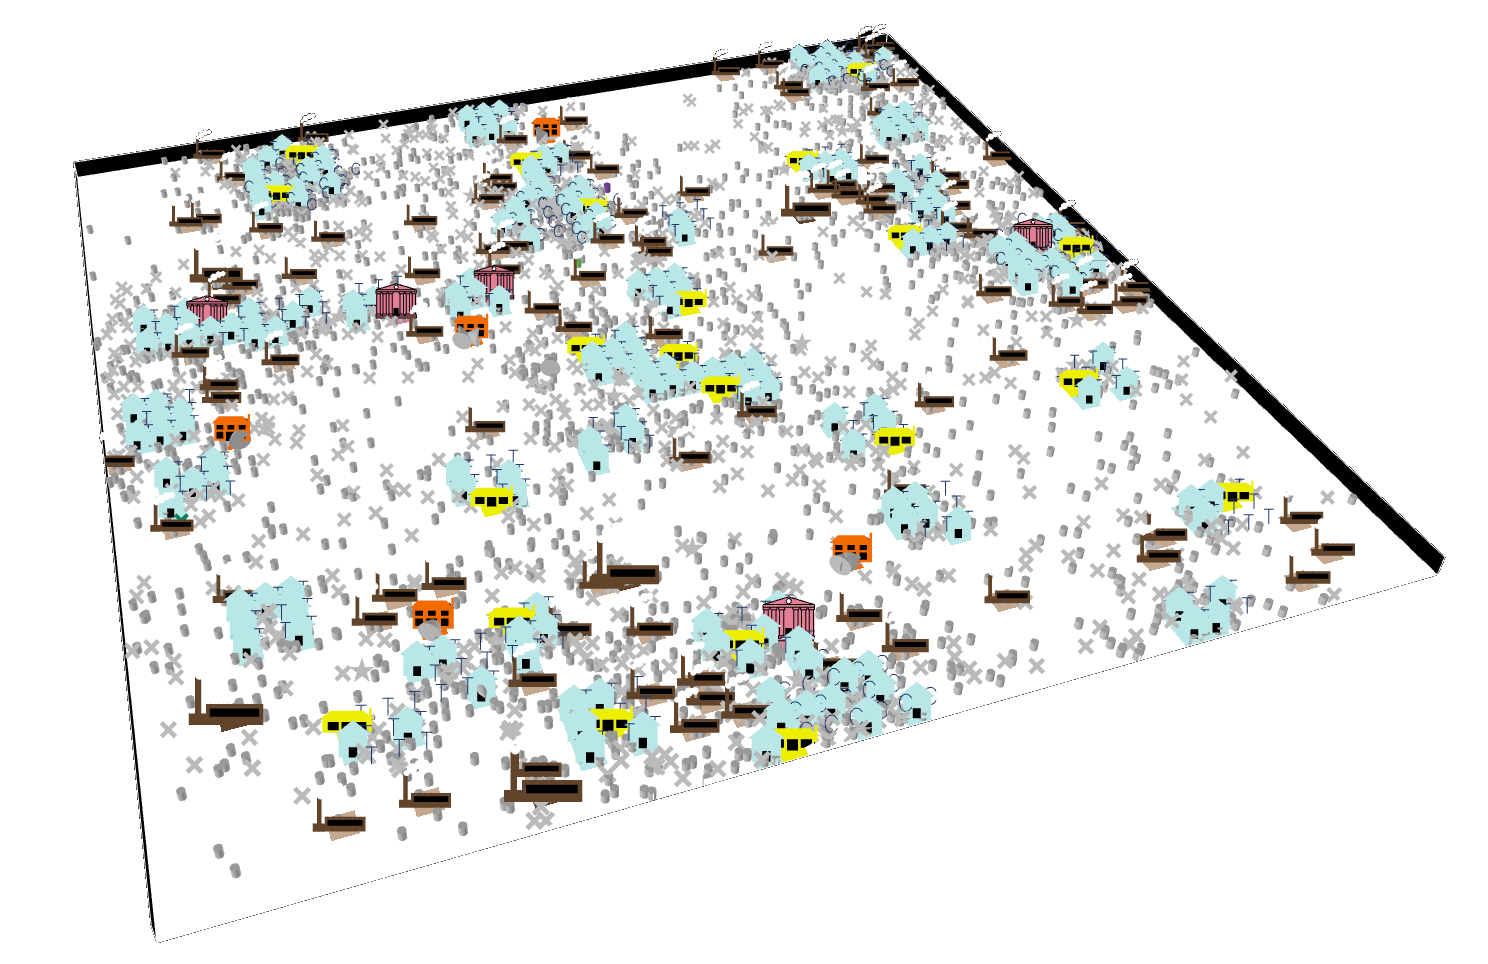
\includegraphics[width=0.9\textwidth,,angle=0]{3D.png}}
\caption{A 3D representation of the model world}
\label{3D}
\end{figure}


We can set: 
\begin{itemize}
\item min and max duration of the individual infection;

\item the length of the incubation interval;

\item the critical distance, i.e., the radius of the possibility of infection in open air, with a given probability;

\item the correction of that probability, due to the personal characteristics of both active and the passive agents; passive agents, as receivers, can be robust, regular, fragile, and extra fragile.

\end{itemize} 

We have two main types of contagion: (a) within a radius, for people moving around, also if only temporary present in a house/factory/nursing home/hospital (in schools we only have students and teachers); (b) in a given space (room or apartment) for people resident in their home or in a hospital or in a nursing home or being in school or in a working environment.

People in hospitals and nursing homes can be infected in two ways: (a) and (b). Instead, while people are at school, they can only receive the disease from people in the same classroom, where only teachers and students are present, so this is a third infection mechanism (c). In all cases, the personal characteristics of the recipients are decisive.

We remark that workplaces are open to all persons, as clients, vendors, suppliers, external workers can go there. In contrast, schools are mainly reserved for students and school operators and are less affected by contact with other types of agents.

All agents have their home, inside a city, or a town. The agents also have usual places (UPs) where they act and interact, moving around. These positions can be interpreted as free time elective places. When we activate the schools, students and teachers have both UPs and schools; healthcare operators have both UPs and hospitals or nursing homes; finally, workers have both UPs and working places. In each day (or tick of the model), we simulated realistic sequences of actions.




Figure \ref{outline} describes what happens during every \emph{day} in our simulated world, with each day as a sequence of several actions.

\begin{figure}[t]
\center
\fbox{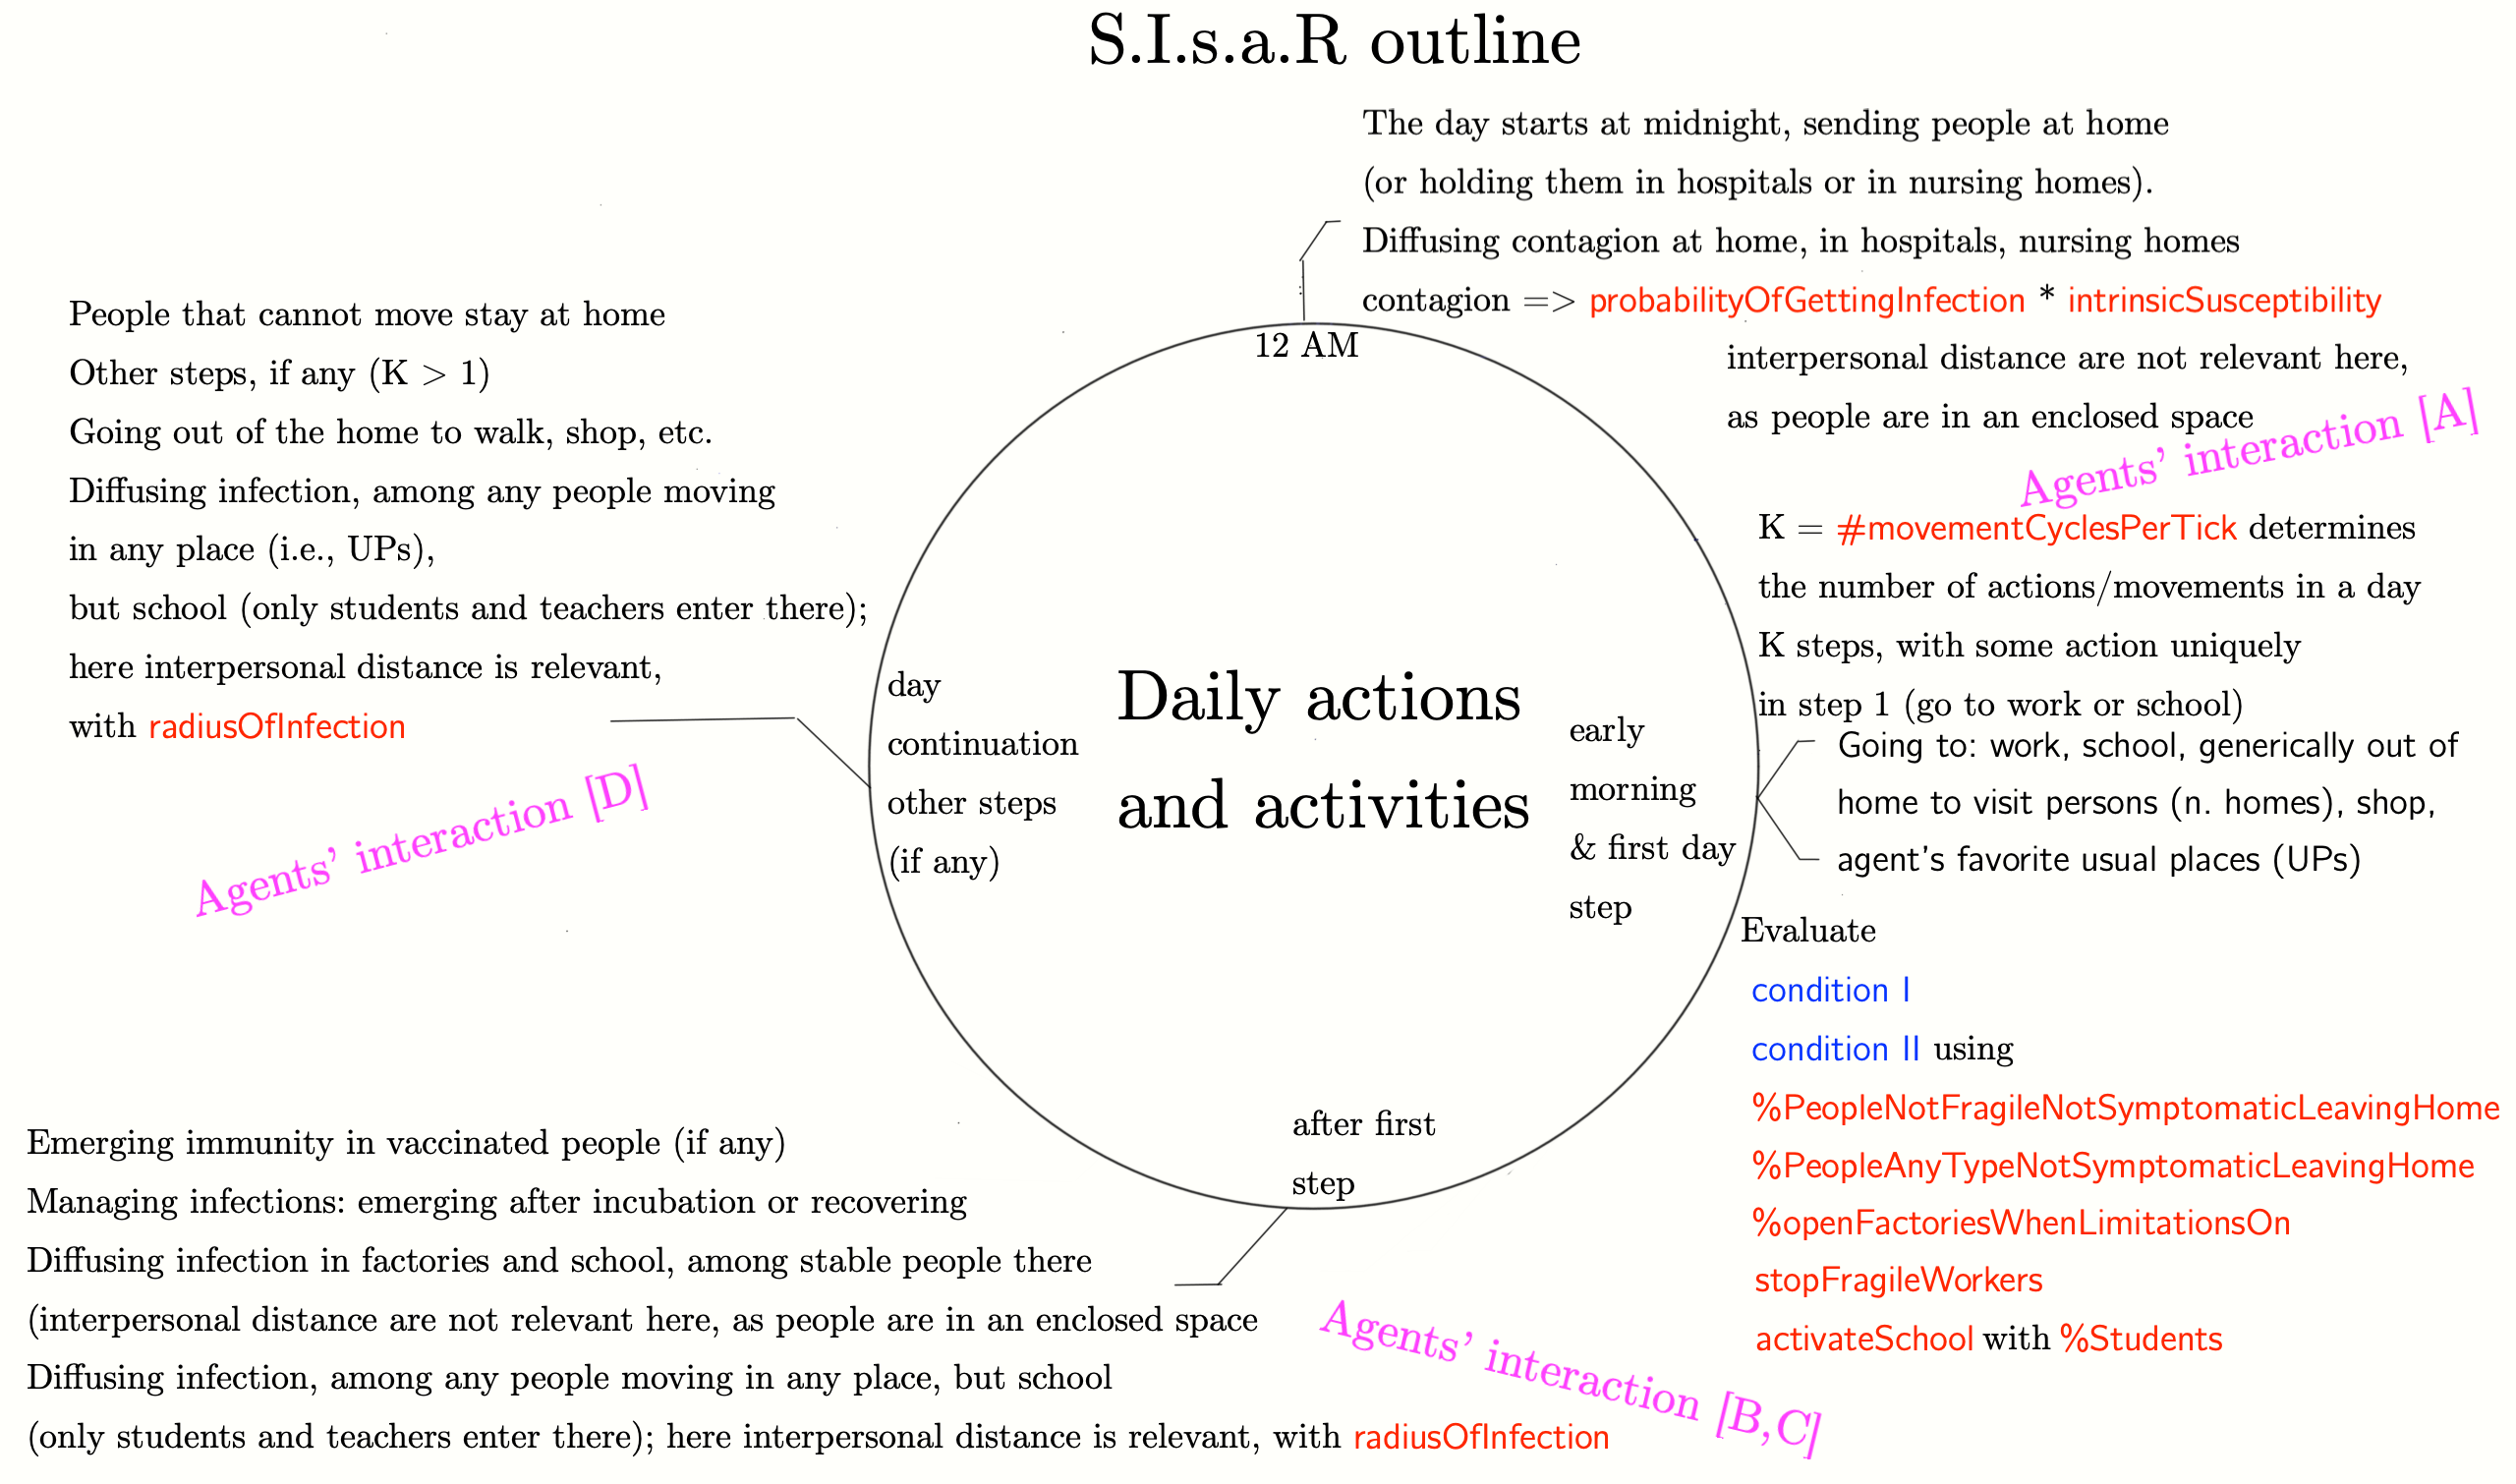
\includegraphics[width=1.3\textwidth,,angle=90]{SIsaR_outline2.png}}
\caption{A day in the simulation, with $N$ repetitions where $N$ is the duration of a specific outbreak; look at: Section \ref{cond} for the rules of the conditional actions; Section \ref{par} for the parameter definitions; and Section \ref{inter} for details on the agent interactions}
\label{outline}
\end{figure}


%%%%%%%%%%%%%%%%%%%%%%%%%%%%%%%%%%%%%%
\subsection{Conditional actions}
\label{cond}

Agents' movements in space, to go to work, school, and other UPs are subject to two interrelated general conditions.

\begin{enumerate}[label=\Roman*]

\item Symptomatic persons are at home or in a hospital or a nursing home and do not move. 

\item People not constrained by \emph{condition I} can move if (primary rule) there are no general limitations (e.g., lockdown) \emph{OR} or one of the following specific sub-conditions applies:

\begin{enumerate}
\item agents who are hospital healthcare operators or nursing home healthcare operators;

\item all people, according to the probability of moving of the whole non-symptomatic agents (\ref{par}, \ref{p3});

\item regular people, according to the probability of moving of the regular non-symptomatic agents
(\ref{par}, \ref{p4});

\item workers, if all the factories are open or it is open their workplace
(\ref{par}, \ref{p5});

\item teachers, if the schools are open
(\ref{par}, \ref{p6});

\item students, if the schools are open, but with a possible quota limitation
(\ref{par}, \ref{p7}).

\end{enumerate}

\end{enumerate}


%%%%%%%%%%%%%%%%%%%%%%%%%%%%%%%%%%%%%%
\subsection{Parameter definition}
\label{par}

We define here the parameters of Figure \ref{outline}, also with the short names used in program scripts, in round brackets. The values of the parameters are reported in detail in Appendix~1~-~Parameter~values (Section \ref{app1}).

\begin{enumerate}[label=\roman*]

\item \label{p1} \emph{probabilityOfGettingInfection} (\verb|prob|) is the base probability of getting infected, to be multiplied by the \emph{intrinsicSusceptibility} factor (\ref{p2}); it is activated if the subject is within a circle of radius  (\ref{p8}) with an infected person; values at (\ref{app1}, \ref{pp1});

\item \label{p2} the \emph{intrinsicSusceptibility} is based on \emph{intrinsicSusceptibilityFactor} set to 5 in Eq. \ref{intrinsic}
\begin{equation}
intrinsicSusceptibility = intrinsicSusceptibilityFactor^{groupFragility}
\label{intrinsic}
\end{equation}
with $groupFragility$ exponent set to:

\begin{description}
\item [1] for extra-fragile persons,
\item [0] for fragile persons,
\item [-1] for regular persons,
\item [-2] young people from 0 to 24 years old;
\end{description}

\item \label{p3} \emph{\%PeopleAnyTypeNotSymptomaticLeavingHome} (\verb|%PeopleAny|)
determines, in a probabilistic way, the number of people of any kind going around in case of limitations/lockdown; the limitations operate only if the lockdown is on (into our simulated world, from day 20); values at (\ref{app1}, \ref{pp3}); 

\item \label{p4} \emph{\%PeopleNotFragileNotSymptomaticLeavingHome} (\verb|%PeopleNot|)
determines, in a probabilistic way, the number of regular people going around in case of limitations/lockdown;
as above, the limitations operate only if the lockdown is on (into our simulated world, from day 20); values at (\ref{app1}, \ref{pp4});

the parameters \ref{p3} and \ref{p4} in some time interval change very frequently, reproducing into the model the uncertainty of the decisions that were happening  in the real world in the same periods; 

NB, the parameters \ref{p3} and \ref{p4} produce independent effects, as in the following examples: (a) the activation of \emph{\%PeopleAny at 31, 0} and, simultaneously, of \emph{\%PeopleNot at 31, 80}, means that people had to stay home on that day, but people specifically not fragile could go out in 80\% of the cases; (b) \emph{\%PeopleAny at 339, 80} and, simultaneously, \emph{\%PeopleNot at 339, 100} means that fragile and not fragile persons cannot always go around, but only in the 80\% of the cases; instead, considering uniquely non-fragile persons they are free to go out; the construction is an attempt to reproduce a fuzzy situation;

in future versions of the model, we will define the quotas more straightforwardly:
\begin{itemize}
\item \verb|%FragilePeopleNotSymptomaticLeavingHome|;
\item \verb|%NotFragilePeopleNotSymptomaticLeavingHome|;
\end{itemize}

\item \label{p5} \emph{\%openFactoriesWhenLimitationsOn} (\verb|%Fac|) 
determines, in a probabilistic way, what factories (small and large industries, commercial surfaces, private and government offices)
are open when limitations are on; if the factory of a worker is open, the subject can go to work, avoiding restrictions (but uniquely in the first step of activity of each day); values at (\ref{app1}, \ref{pp5}); 

\item \label{p6} \emph{stopFragileWorkers}  (\verb|sFW|) is \emph{off} (set to 0) by default; if \emph{on} (set to 1), fragile workers (i.e., people fragile due to prior illnesses) can move out of their homes following the \ref{p3} and \ref{p4} parameters, but cannot go to work; the regular case is that the workers (fragile or regular) can go to their factory (if open) also when limitations are on; values at (\ref{app1}, \ref{pp6});

alternatively, we also have the \verb|fragileWorkersAtHome| parameter; if \emph{on} (set to 1) the total of the workers is unchanged, but the workers are all regular; we can activate this counterfactual operation uniquely at the beginning of the simulation;

\item \label{p7} when \emph{activateSchools} (\verb|aSch|) is \emph{on} (set to 1), teachers and students go to school avoiding restrictions (but uniquely in the first step of activity of each day); \emph{\%Students} (\verb|%St|) limits to its value the quota of the students moving to school; the residual part is following the lessons from home; values at (\ref{app1}, \ref{pp7});

\item \label{p8} following \emph{radiusOfInfection} (\verb|radius|), the effect of the contagion---outside enclosed spaces, or there, but for temporary presences---is possible within that distance; values at (\ref{app1}, \ref{pp8}).

\end{enumerate}

%%%%%%%%%%%%%%%%%%%%%%%%%%%%%%%%%%%%%%
\subsection{Agents' interaction}
\label{inter}

We underline that our simulation tool is not based on micro-simulation sequences, calculating the contagion agent by agent, on the base of their characteristics and ex-ante probabilities. It implements a true agent-based simulation, with the agents acting and, most of all, interacting, thus generating continuously contagion situations.

Each run creates a population with expected characteristics, but also with random specifications, to assure the heterogeneity in agents. The daily choices of the agents are partially randomized, to reproduce real-life variability.

Contagions arise from agents' interactions, in four situations, as specified in Fig. \ref{outline}:

\begin{enumerate}[label=\Alph*]

\item - in houses (at night), hospitals, nursing homes;

\item - in schools, workplaces in general, among people stable there;

\item - in the places above (excluding schools) by people temporary there and in open spaces (UPs above);

\item - interactions mainly in open spaces (UPs above).

\end{enumerate}

%%%%%%%%%%%%%%%%%%%%%%%%%%%%%%%%%%%%%%%%%%%%%%%%%%%%%%%%%
\section{Contagion representation}

P R O V V I S O R I O

collegare a Appendix~2~-~A gallery of contagion sequences (Section \ref{app2})

  \begin{itemize}
  \item
The model allows analyzing the sequences of contagions in simulated epidemics, reporting the places where the contagion occur. 
  \item
We represent each infected agent as a horizontal segment (from the starting date to the final date of the infection) with vertical connections to other agents if they receive the disease.

We represent the new infected agents via further segments at an upper level. 

  \item
With colors, line thickness, and styles, we display multiple information. 

  \item
This enables understanding at a glance how an epidemic episode is developing. In this way, it is easier to reason about countermeasures and, thus, to develop intervention policies.

  \end{itemize}

Examples.

\begin{figure}[t]
\center
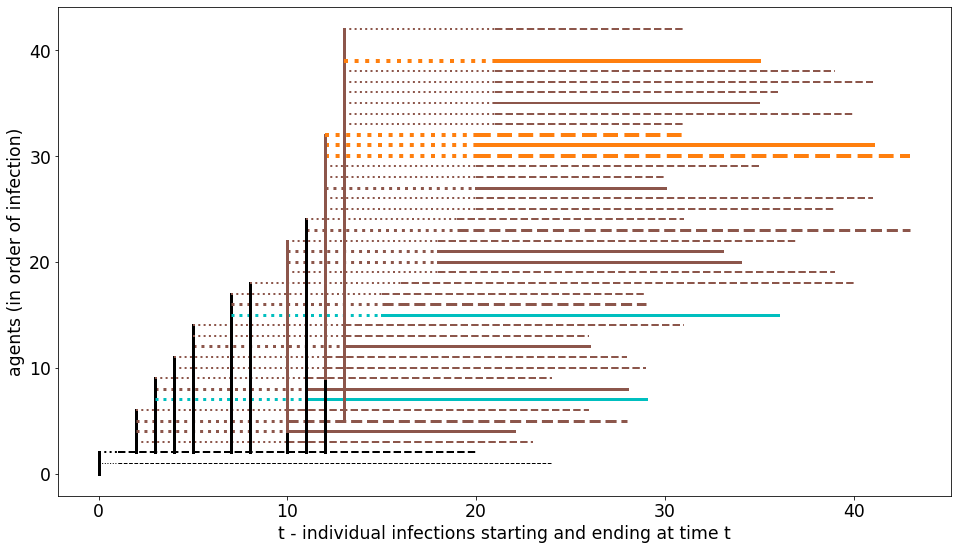
\includegraphics[width=0.9\textwidth]{with8b40.png}% with control case 473323 474697 in SIsaR_0.9.4.1 experiments 2 seeds with control-table_10000.csv, file withControl_473323_474697.csv
\caption{A case with containment measures, first 40 infections: workplaces (brown) and nursing homes (orange) strictly interweaving}
\label{workplacesNursingHomes}
\end{figure}


\begin{figure}[t]
\center
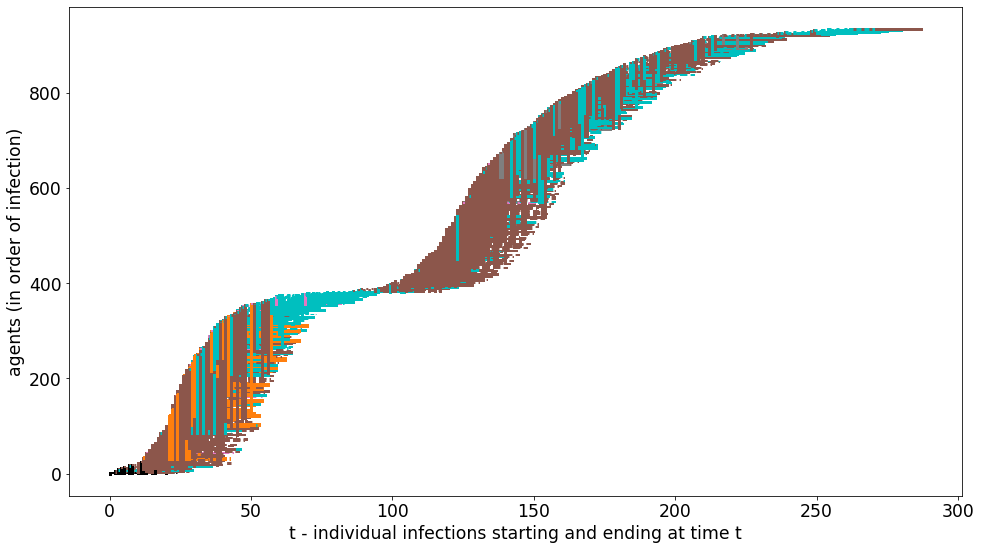
\includegraphics[width=0.9\textwidth]{with8a.png}% with control case 473323 474697 in SIsaR_0.9.4.1 experiments 2 seeds with control-table_10000.csv, file withControl_473323_474697.csv
\caption{A Case with containment measures, the whole epidemics: workplaces (brown) and nursing homes (orange) and then houses (cyan), with a bridge connecting two waves}
\label{workplacesNursingHomesFull}
\end{figure}


%%%%%%%%%%%%%%%%%%%%%%%%%%%%%%%%%%%%%%%%%%%%%%%%%%%%%%%%%
\section{Exploring cases}

%%%%%%%%%%%%%%%%%%%%%%%%%%%%%%%%%%%%%%%%%%%%%%%%%%%%%%%%%
\subsection{Simulation batches}

%%%%%%%%%%%%%%%%%%%%%%%%%%%%%%%%%%%%%%%%%%%%%%%%%%%%%%%%%
\subsection{Epidemics without and with control}

%%%%%%%%%%%%%%%%%%%%%%%%%%%%%%%%%%%%%%%%%%%%%%%%%%%%%%%%%
\subsection{Actual data}

%%%%%%%%%%%%%%%%%%%%%%%%%%%%%%%%%%%%%%%%%%%%%%%%%%%%%%%%%
\section{Factual and counterfactual analyses}


%%%%%%%%%%%%%%%%%%%%%%%%%%%%%%%%%%%%%%%%%%%%%%%%%%%%%%%%%
\subsection{Spontaneous second wave, without specific measures}

%%%%%%%%%%%%%%%%%%%%%%%%%%%%%%%%%%%%%%%%%%%%%%%%%%%%%%%%%
\subsection{Second wave, new infections from outside, without specific measures}

%%%%%%%%%%%%%%%%%%%%%%%%%%%%%%%%%%%%%%%%%%%%%%%%%%%%%%%%%
\subsection{Here a Stefano's section on calculating the infection indicator without delays }

%%%%%%%%%%%%%%%%%%%%%%%%%%%%%%%%%%%%%%%%%%%%%%%%%%%%%%%%%
\subsection{Second wave, new infections from outside, with new specific measure anticipation of -20 days}

N.B.: (i) anticipation limit Oct 5.; (ii) also the ending date of each measure is anticipated of 20 days.

%%%%%%%%%%%%%%%%%%%%%%%%%%%%%%%%%%%%%%%%%%%%%%%%%%%%%%%%%
\subsection{Second wave, new infections from outs., stop fragile people. 60  days from Oct. 5}

Schools are always working 100\% in this case.

%%%%%%%%%%%%%%%%%%%%%%%%%%%%%%%%%%%%%%%%%%%%%%%%%%%%%%%%%
\subsection{To recap}

%%%%%%%%%%%%%%%%%%%%%%%%%%%%%%%%%%%%%%%%%%%%%%%%%%%%%%%%%
\section{Planning vaccination campaigns}

\subsection{Here an Alberto's section on \emph{How vaccines work}}

%%%%%%%%%%%%%%%%%%%%%%%%%%%%%%%%%%%%%%%%%%%%%%%%%%%%%%%%%
\subsection{Planning a vaccination campaign using GAs (with non-pharmaceutical containment measures in action)}

\subsubsection{Vaccination groups}

We take into consideration seven groups in order of decreasing fragility but also considering the exposure to contagion:

\begin{enumerate}
\item [\emph{g1}]
	extra fragile people with three components;
	\begin{itemize}
		\item due to intrinsic characteristics: people in nursing homes;
		\item due to risk exposure:
		\begin{itemize}
			\item nursing homes operators;
			\item healthcare operators;
 		\end{itemize} 
 	\end{itemize}  
\item [\emph{g2}]
	teachers;
\item [\emph{g3}]
	workers with medical fragility;
\item [\emph{g4}]
	regular workers;
\item [\emph{g5}]
	fragile people without special characteristics;
\item [\emph{g6}]
	regular people, not young, not worker, and not teacher;
\item [\emph{g7}]
	young people excluding special activity cases (a limited number in \emph{g1}).
\end{enumerate}


%%%%%%%%%%%%%%%%%%%%%%%%%%%%%%%%%%%%%%%%%%%%%%%%%%%%%%%%%
\subsection{A specific realistic case}

%%%%%%%%%%%%%%%%%%%%%%%%%%%%%%%%%%%%%%%%%%%%%%%%%%%%%%%%%
\subsection{Vaccination quotas, \emph{plain} strategy}


%%%%%%%%%%%%%%%%%%%%%%%%%%%%%%%%%%%%%%%%%%%%%%%%%%%%%%%%%
\subsection{Vaccination quotas, \emph{wise} strategy}



%%%%%%%%%%%%%%%%%%%%%%%%%%%%%%%%%%%%%%%%%%%%%%%%%%%%%%%%%
\subsection{GAs quotas in the experiment, with vac. people spreading or not spreading the infection}


%%%%%%%%%%%%%%%%%%%%%%%%%%%%%%%%%%%%%%%%%%%%%%%%%%%%%%%%%
\subsection{An experiment with GA}

%%%%%%%%%%%%%%%%%%%%%%%%%%%%%%%%%%%%%%%%%%%%%%%%%%%%%%%%%
\subsubsection{Time dynamics without vaccinations}

%%%%%%%%%%%%%%%%%%%%%%%%%%%%%%%%%%%%%%%%%%%%%%%%%%%%%%%%%
\subsubsection{Time dynamics with \emph{plain} vac. strategy, vac. people still spreading the infection}

%%%%%%%%%%%%%%%%%%%%%%%%%%%%%%%%%%%%%%%%%%%%%%%%%%%%%%%%%
\subsubsection{Time dynamics with \emph{wise} vac. strategy, vac. people still spreading the infection}

%%%%%%%%%%%%%%%%%%%%%%%%%%%%%%%%%%%%%%%%%%%%%%%%%%%%%%%%%
\subsubsection{Time dynamics with best GAs strategy, vac, people still spreading the infection}


%%%%%%%%%%%%%%%%%%%%%%%%%%%%%%%%%%%%%%%%%%%%%%%%%%%%%%%%%
\section{A new model and future developments}

%%%%%%%%%%%%%%%%%%%%%%%%%%%%%%%%%%%%%%
\section{Appendix 1 - Parameter values}
\label{app1}

We report here the values of parameters of Figure \ref{outline}, also with the short names used in program scripts, in round brackets. Look at Section \ref{par} for the definition. Day numbering is related to actual dates via the Table \ref{dates}. Day 1 is fixed at Feb \nth{4}, 2020.

The values adopted in the experiments reported in this work are the following.

\begin{enumerate}[label=\roman*]

\item \label{pp1} The values of \emph{probabilityOfGettingInfection} (\verb|prob|) are: 0.05 (starting phase); 0.02 at day 49 (adoption of non-pharmaceutical measures); 0.035 at day 149 (some relaxation in compliance); 0.02 at day 266 (again, compliance to rules).  

\item \label{pp2} \emph{intrinsicSusceptibility} is set discussing Eq. \ref{intrinsic} in (\ref{par}, \ref{p2}).

\item \label{pp3} The values of \emph{\%PeopleAnyTypeNotSymptomaticLeavingHome} (\verb|%PeopleAny|) are:
at (day) 20, 90; at 28, 80; at 31, 0; at 106, 80; at 110, 95; at112, 85; at 117, 95; at 121, 90; at 259, 90; at 266, 80; at 277, 50;
at 302, 70; at 320, 90; at 325, 50; at 329, 80; at 332, 50; at 336, 80; at 337, 50; at 339, 80; 

\item \label{pp4} The values of \emph{\%PeopleNotFragileNotSymptomaticLeavingHome} (\verb|%PeopleNot|) are:
at (day) 31, 80; at 35, 70; at 36, 65; at 38, 15; at 42, 25; at 84, 30; at 106, 0; at 302, 90; at 325, 50; at 332, 50; 
at 337, 50; at 339, 100; at 349, 90;

\item \label{pp5} The values of \emph{\%openFactoriesWhenLimitationsOn} (\verb|%Fac|) are:
at (day) 38, value4 0; at 49, 20; at 84, 70; at 106, 100; at 266, 90; at 277, 70; at 302, 80; at 320, 90; at 325, 30;
at 329, 90; at 332, 30; 336, 90; at 337, 30; at 339, 100;

\item \label{pp6} \emph{stopFragileWorkers}  (\verb|sFW|): by default, 0; in one of the experiments we used \verb|sFW| with set to 1 (on) at day 245  and to 0 (off) at day 275;

\item \label{pp7} The values of \emph{activateSchools} (\verb|aSch|) are:
at (day) 1, on; at 17, off; at 225, on; at 325, off; at 339, on; 

the values of  \emph{\%Students} (\verb|%St|) are: 
at (day) 0, 100; at 277, 50; at 339, 50; at 350, 50 (repeated values are not relevant for the model, but for the use of the programmer-author);

\item \label{pp8} The value of \emph{radiusOfInfection} (\verb|radius|) is 0.2; in the model, space is missing of a scale, but forcing the area to be in the scale of a region as Piedmont, 0.2 is equivalent to 20 meters; we have to better calibrate this measure with movements and probabilities; this is a critical step in future developments of the model.

\end{enumerate}




\begin{table}[t]
\begin{center}
\begin{footnotesize}
\begin{tabular}{rrrrrrrrrrr}
\hline\noalign{\smallskip}
 Day & Date  &~~~~~~~~& Day & Date &~~~~~~~~& Day & Date &~~~~~~~~& Day & Date \\
 \noalign{\smallskip}\svhline\noalign{\smallskip}
 25 & 28- 2-2020 & & 200 & 21- 8-2020 & & 375 & 12- 2-2021 & & 550 &  6- 8-2021 \\
 50 & 24- 3-2020 & & 225 & 15- 9-2020 & & 400 &  9- 3-2021 & & 575 & 31- 8-2021 \\
 75 & 18- 4-2020 & & 250 & 10-10-2020 & & 425 &  3- 4-2021 & & 600 & 25- 9-2021 \\
100 & 13- 5-2020 & & 275 &  4-11-2020 & & 450 & 28- 4-2021 & & 625 & 20-10-2021 \\
125 &  7- 6-2020 & & 300 & 29-11-2020 & & 475 & 23- 5-2021 & & 650 & 14-11-2021 \\
150 &  2- 7-2020 & & 325 & 24-12-2020 & & 500 & 17- 6-2021 & & 675 &  9-12-2021 \\
175 & 27- 7-2020 & & 350 & 18- 1-2021 & & 525 & 12- 7-2021 & & 700 &  3- 1-2022 \\
\hline\noalign{\smallskip}
\end{tabular}
\end{footnotesize}
\caption{The days of the simulation and their equivalent dates in the calendar}
\label{dates}
\end{center}
\end{table}


%%%%%%%%%%%%%%%%%%%%%%%%%%%%%%%%%%%%%%
\section{Appendix 2 - a gallery of contagion sequences}
\label{app2}

A gallery of contagion sequences in Table \ref{gallery}.

    \begin{table}
        \centering
        \begin{tabular}{cccc}
           \hline\noalign{\smallskip}
            Nr. & a & b & c  \\
             \noalign{\smallskip}\svhline\noalign{\smallskip}
1 & 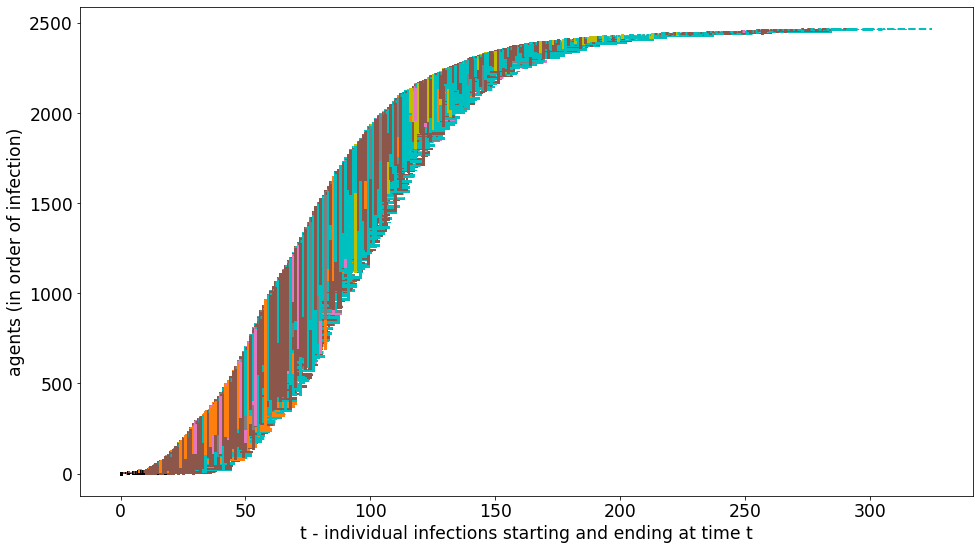
\includegraphics[width=12em]{sequences/no3a.png} & % no control case 10932215 10933923 in SIsaR_0.9.4.1tmp experiments 2 seeds no control-table_5000.csv, file noControl_10932215_10933923.csv
      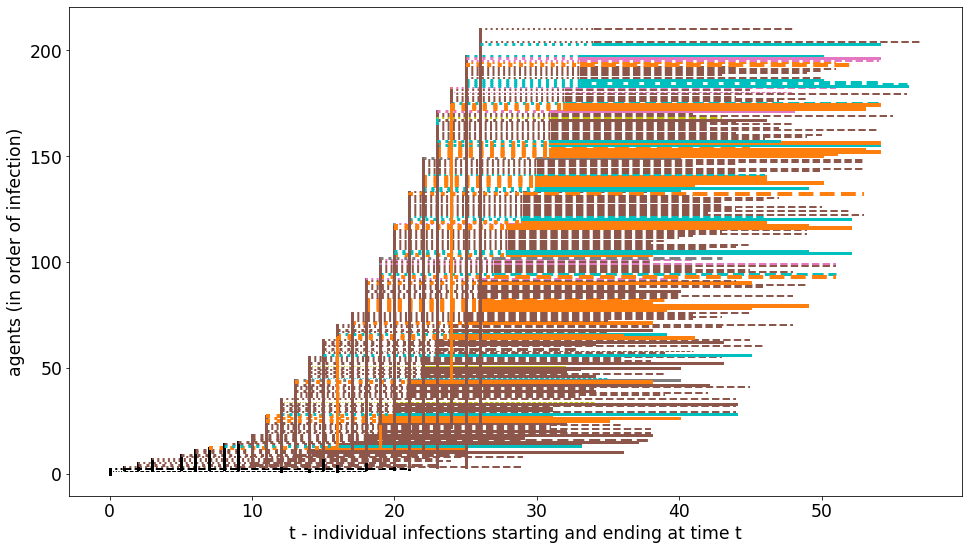
\includegraphics[width=12em]{sequences/no3b.png} & % no control case 10932215_10933923 in SIsaR_0.9.4.1tmp experiments 2 seeds no control-table_5000.csv, file noControl_10932215_10933923.csv
      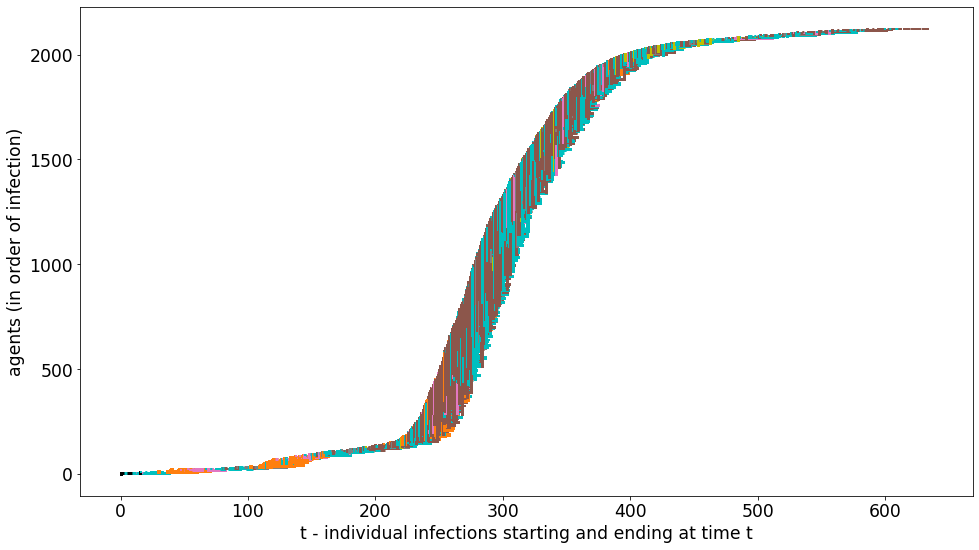
\includegraphics[width=12em]{sequences/no4a.png}    % no control case 12518034 12520144 in SIsaR_0.9.4.1tmp experiments 2 seeds no control-table_5000.csv, file noControl_12518034_12520144.csv
\\
2 & 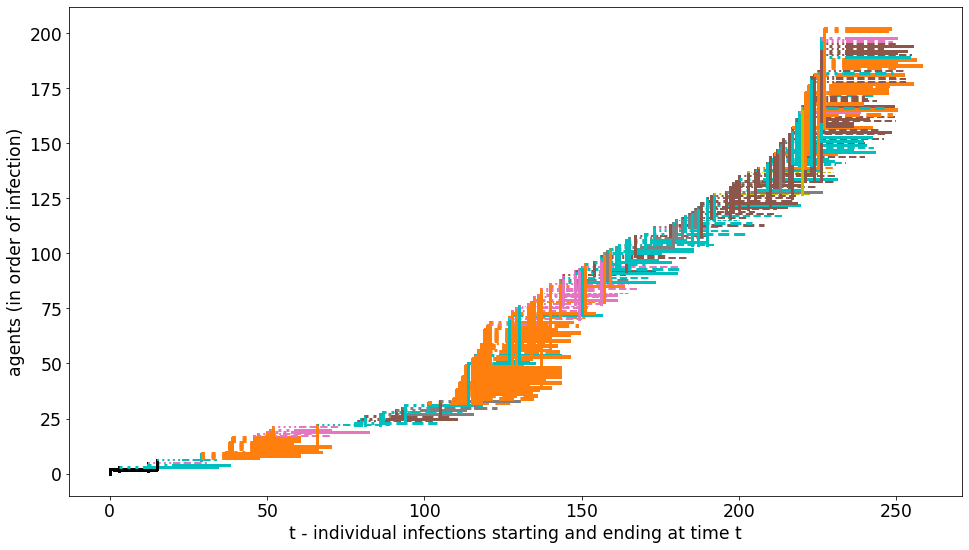
\includegraphics[width=12em]{sequences/no4b.png} & % no control case 12518034 12520144 in SIsaR_0.9.4.1tmp experiments 2 seeds no control-table_5000.csv, filee noControl_12518034_12520144.csv
      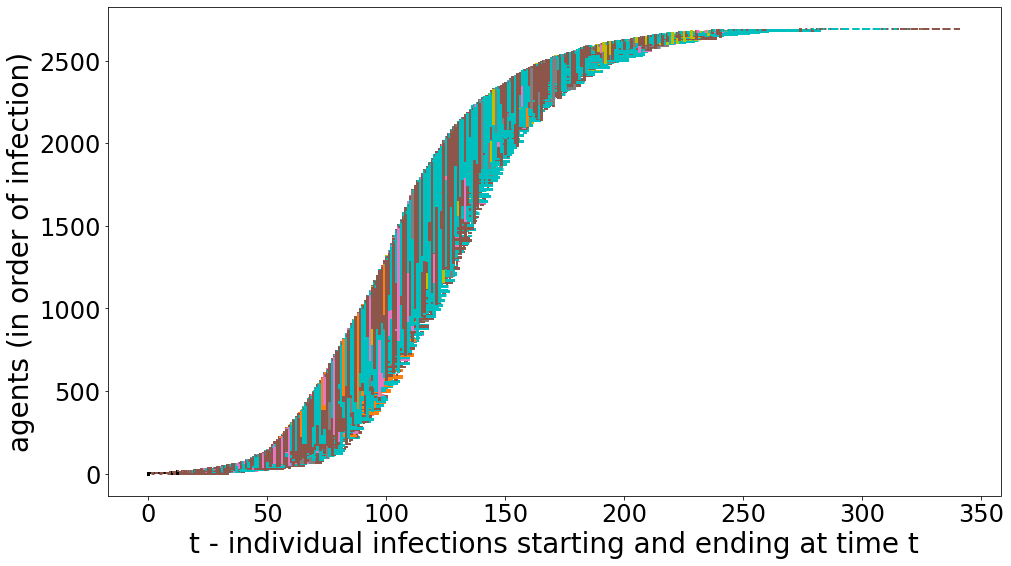
\includegraphics[width=12em]{sequences/no5a.png} & % no control case 113790741 13792228 in SIsaR_0.9.4.1tmp experiments 2 seeds no control-table_5000.csv, file noControl_13790741 13792228.csv
      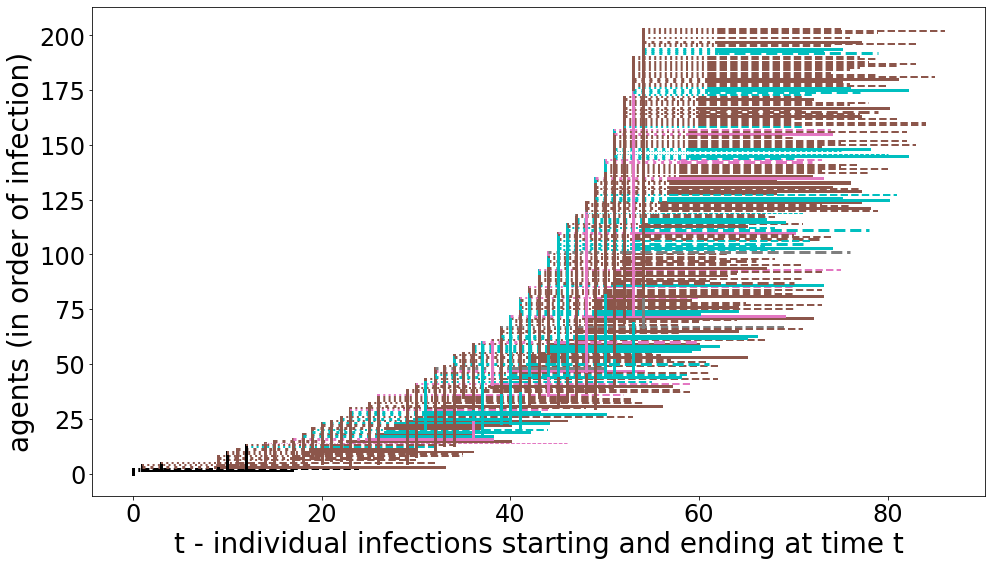
\includegraphics[width=12em]{sequences/no5b.png}    % no control case 113790741 13792228 in SIsaR_0.9.4.1tmp experiments 2 seeds no control-table_5000.csv, file noControl_13790741 13792228.csv
\\
3 & 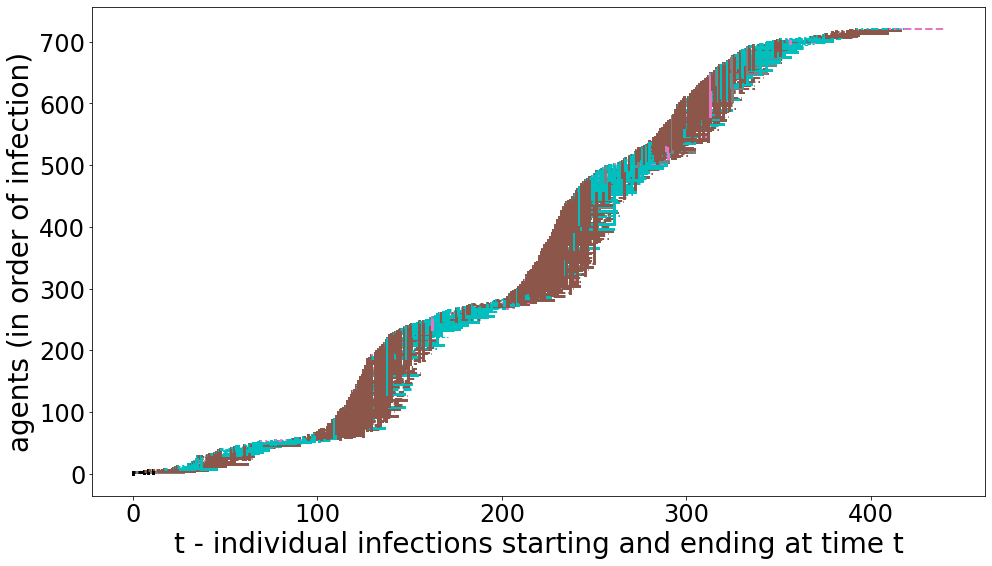
\includegraphics[width=12em]{sequences/with6a.png} & % with control case 268411 270578 in SIsaR_0.9.4.1 experiments 2 seeds with control-table_10000.csv, file withControl_268411_270578.csv
      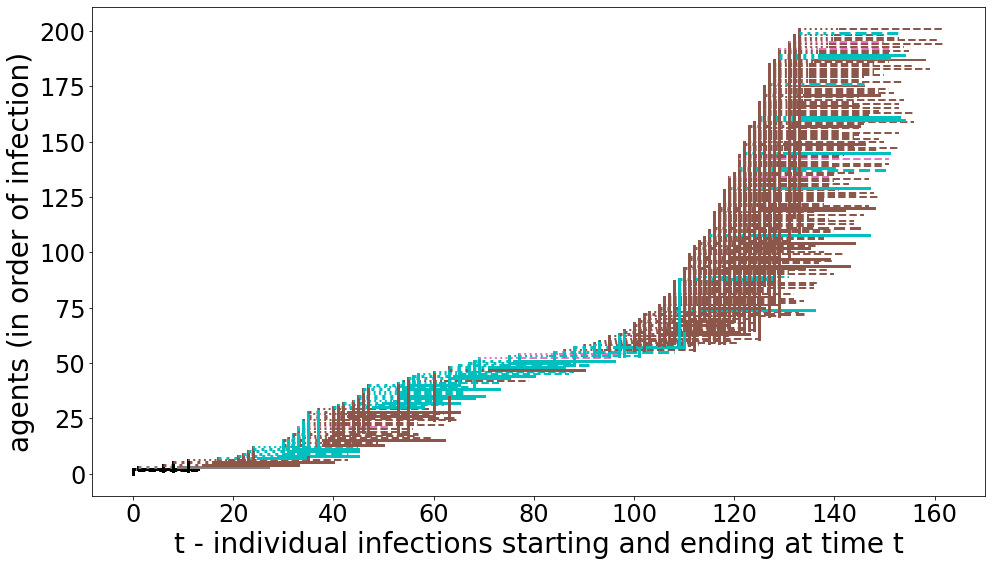
\includegraphics[width=12em]{sequences/with6b.png} & % with control case 268411 270578 in SIsaR_0.9.4.1 experiments 2 seeds with control-table_10000.csv, file withControl_268411_270578.csv
      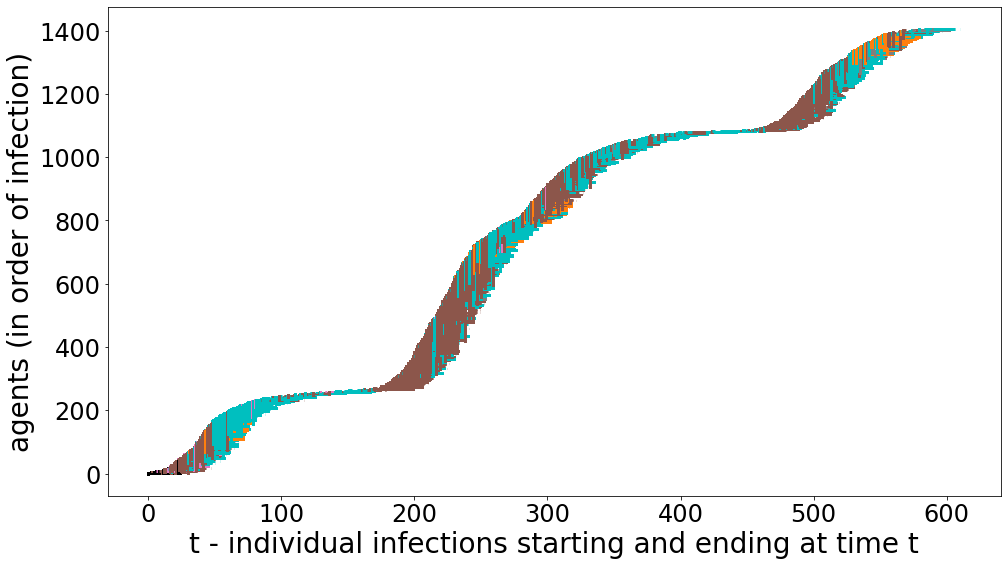
\includegraphics[width=12em]{sequences/with7a.png}    % with control case 2722110 2723664 in SIsaR_0.9.4.1 experiments 2 seeds with control-table_10000.csv, file withControl_2722110_2723664.csv
\\
4 & 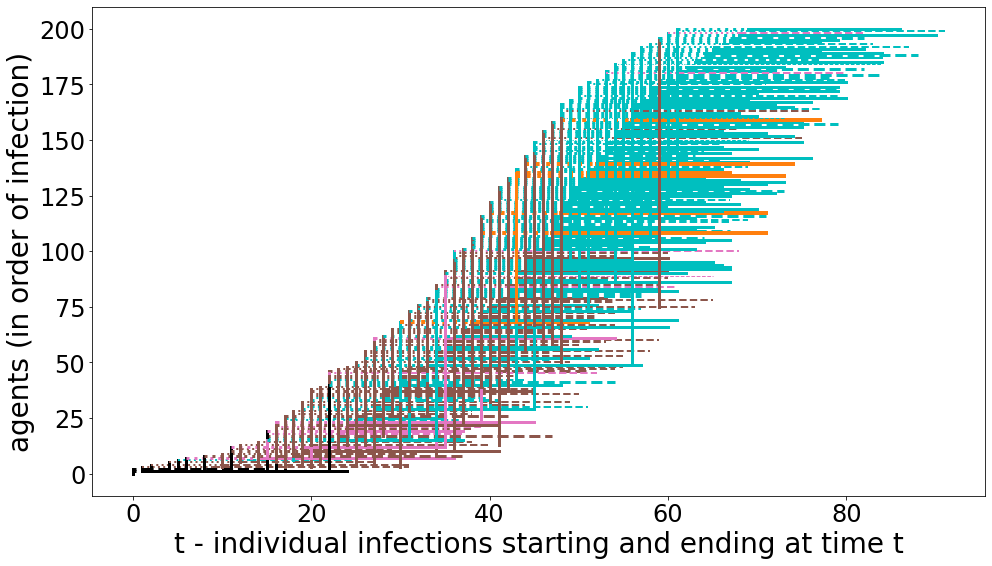
\includegraphics[width=12em]{sequences/with7b.png} & % with control case 2722110 2723664 in SIsaR_0.9.4.1 experiments 2 seeds with control-table_10000.csv, file withControl_2722110_2723664.csv
      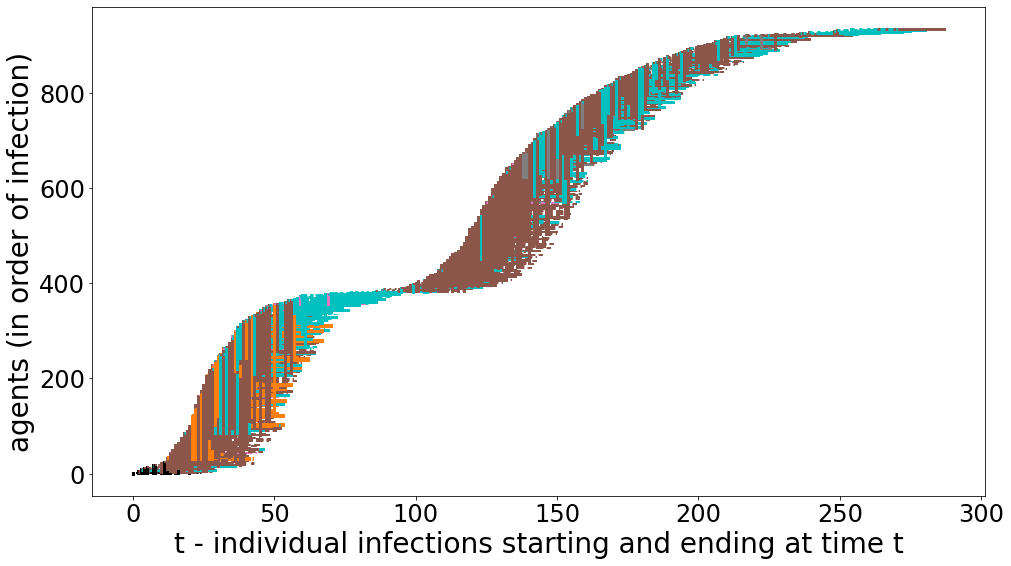
\includegraphics[width=12em]{sequences/with8a.png} & % with control case 473323 474697 in SIsaR_0.9.4.1 experiments 2 seeds with control-table_10000.csv, file withControl_473323_474697.csv
      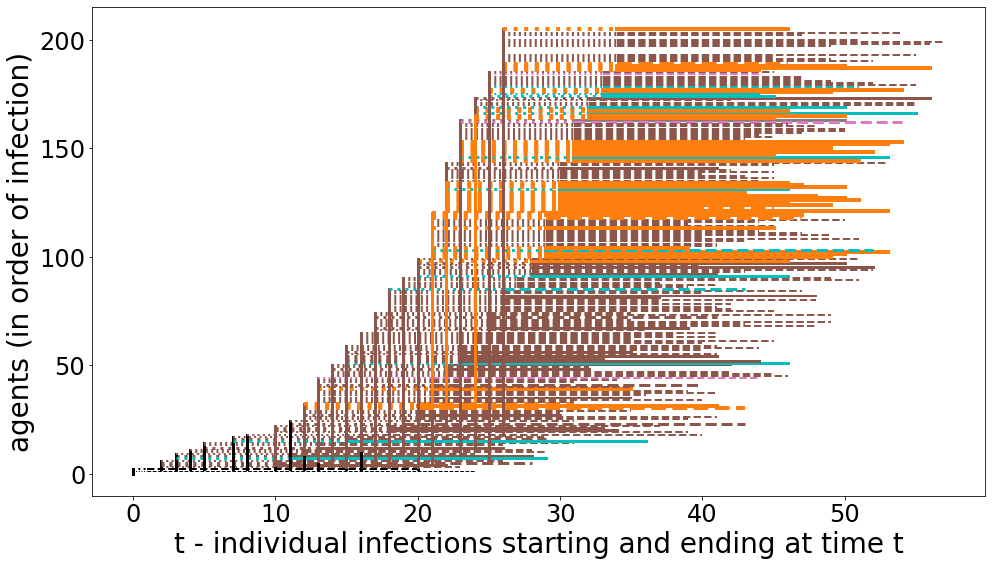
\includegraphics[width=12em]{sequences/with8b.png}    % with control case 473323 474697 in SIsaR_0.9.4.1 experiments 2 seeds with control-table_10000.csv, file withControl_473323_474697.csv
\\
5 & 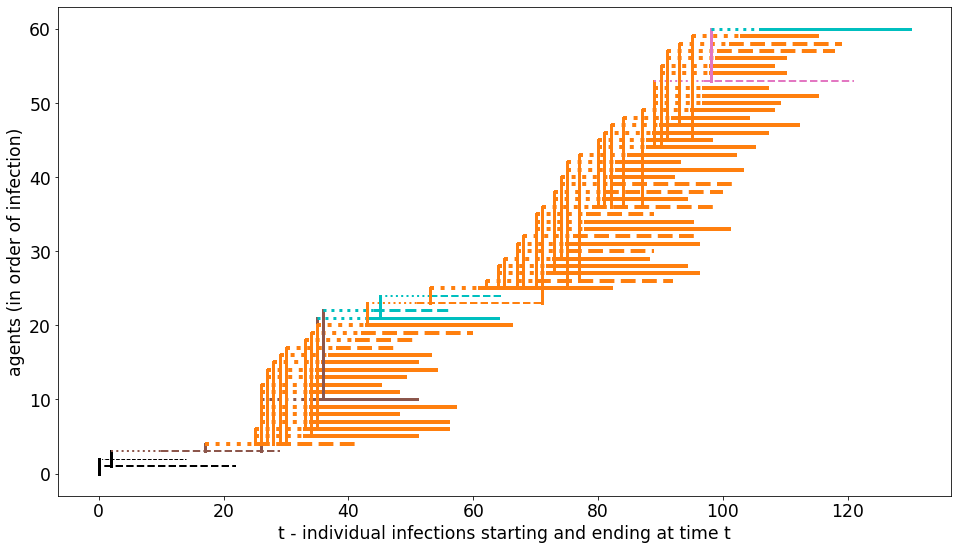
\includegraphics[width=12em]{sequences/withShort0.png} & %using SIsaR 9.4.2 as is (basic control) with 123456_22313, file ex123456_22313.csv
      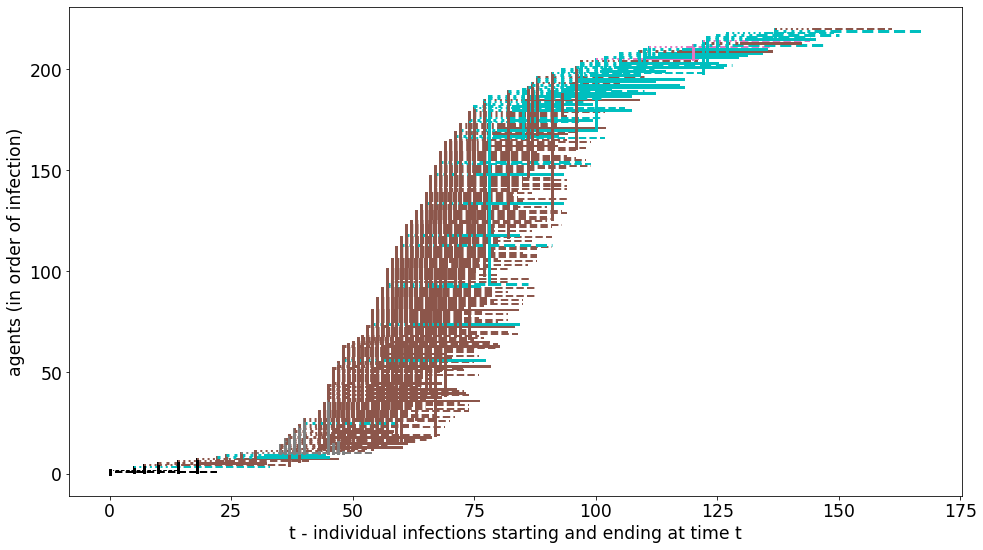
\includegraphics[width=12em]{sequences/withShort1.png} & %using SIsaR 9.4.2 as is (basic control) with 123456_22314
      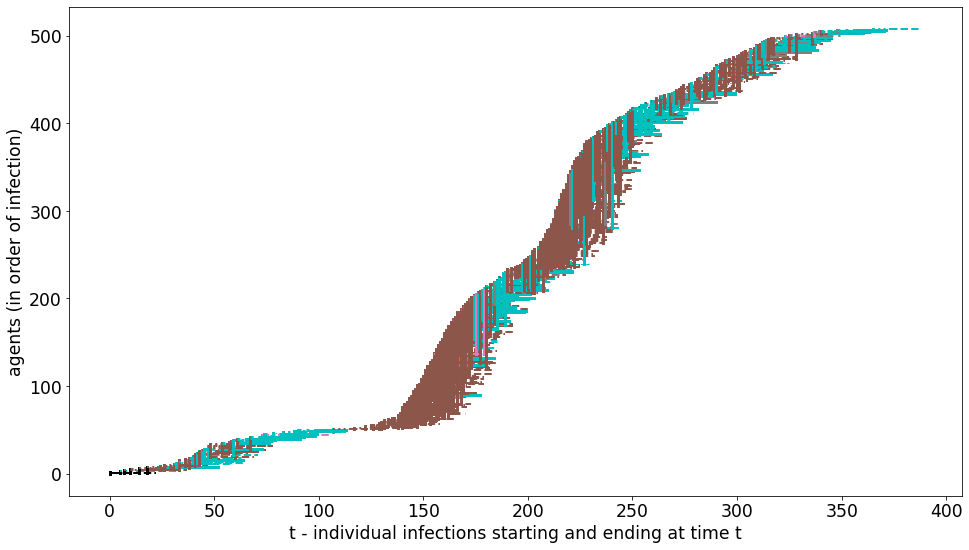
\includegraphics[width=12em]{sequences/withShort1A.png}   %using SIsaR 9.4.2 as is (basic control + 20 sFW 1,i.e., stop Fragile Workers) with 123456_22314
\\
6 & 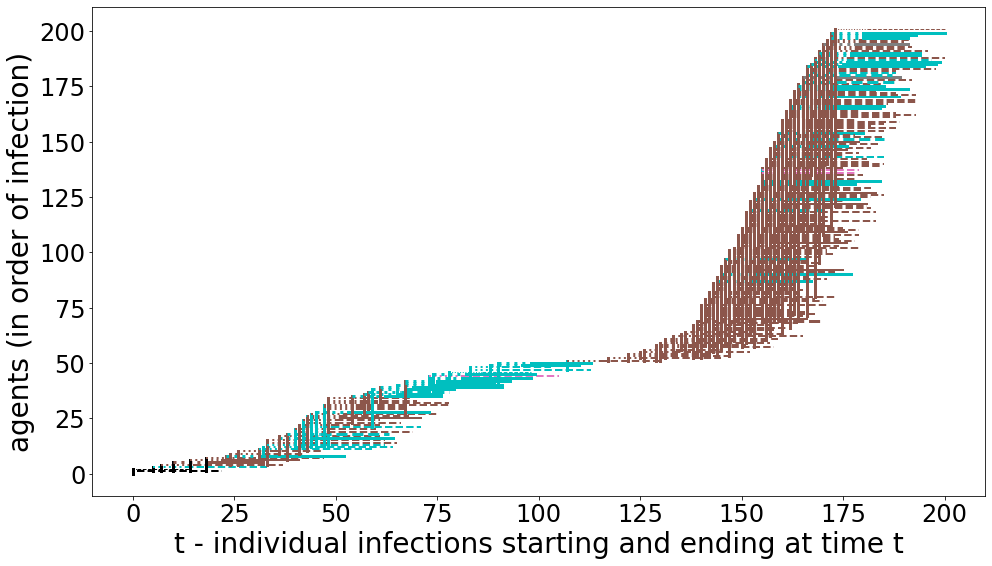
\includegraphics[width=12em]{sequences/withShort1A200.png} & %using SIsaR 9.4.2 as is (basic control + 20 sFW 1,i.e., stop Fragile Workers) with 123456_22314
      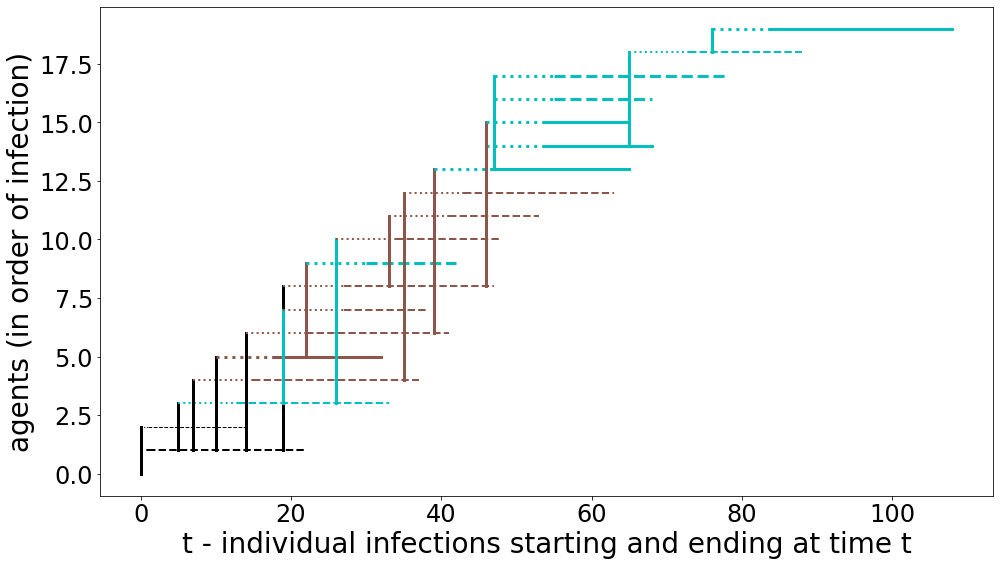
\includegraphics[width=12em]{sequences/withShort1B.png}       & %using SIsaR 9.4.2 as is (basic control + $$$) with 123456_22314
      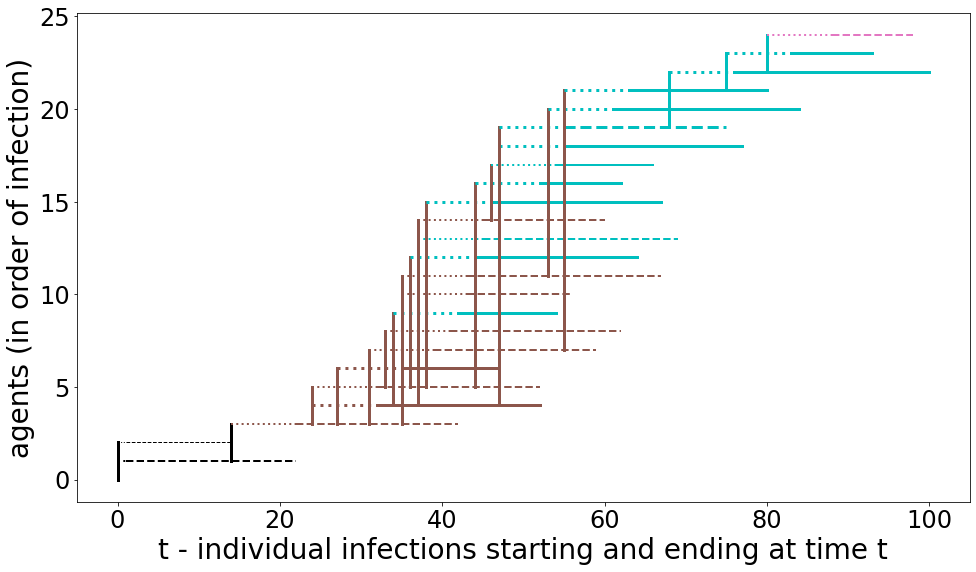
\includegraphics[width=12em]{sequences/withShort2.png}             %using SIsaR 9.4.2 as is (basic control) with 123456_22315, file ex123456_22315.csv123456_22314
\\
           \hline\noalign{\smallskip}
        \end{tabular}
        \caption{Gallery of sequences}
        \label{gallery}
    \end{table}

\begin{itemize}
\item [1a] Case 1, without containment measures: contagions in nursing homes (orange), workplaces (brown), homes (cyan), hospitals (pink)
\item [1b] Case 1, without containment measures, first 200 infections with the main contribution of nursing homes (orange) and workplaces (brown)
\item [1c] Case 2, without containment measures: nursing homes (orange) as starter
\item [2a] Case 2, without containment measures, first 200 infections: nursing homes (orange) as starter and around day 70 a unique contagion at home continuing the epidemic
\item [2b] Case 3, without containment measures: an initial deep effect of contagions in workplaces (brown) and homes (cyan)
\item [2c] Case 3, without containment measures, first 200 infections: the initial deep effect of contagions in workplaces (brown) and homes is due in the initial steps to fragile persons, also asymptomatic
\item [3a] Case 4, with containment measures: another case of strong contribution of workplaces (brown) and homes (cyan) to epidemic diffusion
\item [3b] Case 4, with containment measures, first 200 infections: after day 100 we observe many significant cases of fragile workers diffusing the infection
\item [3c] Case 5, with containment measures: workplaces (brown), hospitals (pink), nursing homes (orange) and homes (cyan), then workplaces
\item [4a] Case 5, with containment measures, first 200 infections: in the beginning workplaces (brown), hospitals (pink), nursing homes (orange) and homes (cyan) interweaving
\item [4b] Case 6, with containment measures: workplaces (brown), nursing homes (orange), homes (cyan)
\item [4c] Case 6, with containment measures, first 200 infections: workplaces (brown) and nursing homes (orange) strictly interweaving
\item [5a] Case 7, with containment measures: the effect of nursing homes (orange)
\item [5b] Case 8, with containment measures: a highly significant effect of workplaces (brown)
\item [5c] Case 8, with containment measures, stopping fragile workers at day 20, with a positive result, but home contagions (cyan) keep alive the pandemic, which explodes again in workplaces (brown)
\item [6a] Case 8, with containment measures, stopping fragile workers at day 20, with a positive effect, but home contagions (cyan) keep alive the pandemic, which explodes again in workplaces (brown), first 200 infections with evidence of the event around day 110 with the new phase due to a unique asymptomatic worker
\item [6b] Case 8, with containment measures, stopping fragile workers and any case of fragility at day 15, also isolating nursing homes
\item [6c] Case 9, with containment measures: a spontaneously stopping epidemic in  short period
\end{itemize}




\bibliography{bibliografiaGenerale}
\bibliographystyle{spphys}

\end{document}
